% Metódy inž7inierskej práce

\documentclass[10pt,oneside,slovak,a4paper]{article}

\usepackage[slovak]{babel}
%\usepackage[T1]{fontenc}
\usepackage[IL2]{fontenc} % lepšia sadzba písmena Ľ než v T1
\usepackage[utf8]{inputenc}
\usepackage{graphicx}
\usepackage{url} % príkaz \url na formátovanie URL
\usepackage{hyperref} % odkazy v texte budú aktívne (pri niektorých triedach dokumentov spôsobuje posun textu)

\usepackage{cite}
%\usepackage{times}

\pagestyle{myheadings}

\title{Možnosti a efektívnosť získania jazykových znalostí prostredníctvom
e-learningu\thanks{Semestrálny projekt v predmete Metódy inžinierskej práce, ak. rok 2020/21, vedenie: Ing. Fedor Lehocki }} % meno a priezvisko vyučujúceho na cvičeniach

\author{Richard Szarka\\[2pt]
	{\small Slovenská technická univerzita v Bratislave}\\
	{\small Fakulta informatiky a informačných technológií}\\
	{\small \texttt{xszarkar@stuba.sk}}
	}

\date{\small 7. október 2020} % upravte



\begin{document}

\maketitle

\begin{abstract}
Získavanie vedomostí cez internet je čoraz bežnejšie. Jednou z najžiadanejších oblastí v e-learningu je najmä získavanie jazykových znalostí. Na osvojenie si jazyka v kontaktnom vzdelávaní je potrebné precvičovať jazyk rôznymi metódami rovnako ako pri autonómnom vzdelávaní pomocou e-learningu. Cieľom tejto práce je definovať a porovnať metódy nadobúdania jazykových zručností prostredníctvom e-learningu. V práci si rozoberieme metódy, ako napríklad úlohy zadávané softwarom (Duolingo), aktívnu komunikáciu s osobou, ktorá daný jazyk už ovláda (Tandem, HelloTalk) alebo pasívnu komunikáciu so skupinou ľudí s rovnakým cieľom (jazykové blogy). Zameriame sa na to, aké výhody majú jednotlivé metódy, ktoré konkrétne jazykové zručnosti rozširujú, ale aj aká je efektívnosť nadobúdania jazykových znalostí cez e-learning.
\end{abstract}

\section{Úvod} %1 uvod

\section{Čo je e-learning?}%2
Učenie sa v dnešnej dobe je tak jednoduché, že stačí na to použitie hocijakého komunikačného zariadenia, ktoré vám je schopné dávať informácie\cite{vyhody}. Pojem e-learning je bežne vysvetlený ako vedomé použitie kominikačných a sieťových technológií v učení a učení sa. Alternatívnou definiciou e-learningu môže byť: aplikovanie elektronických systémov, ako internet a pocitace, ktoré šetria čas a financie \cite{efektivnost}. 

\subsection{Výhody e-learningu}%2.1
Ku každej novej technológii patria výhody. E-learning priniesol mnohé výhody v učení a výučby, ktoré zahrňujú aj výučbu jazykov. Medzi mnohé z výhod patrí:
\begin{itemize}
\item E-learning je rýchly a dynamický a znižuje výdavky (ako napríklad cestovanie) \cite{efektivnost}
\item Lekcie sú pripravované rôznými učiteľmi \cite{efektivnost}
\item Interaktívne cvičenia zvyšujú motiváciu študentov \cite{vyhody}
\item Aktivity e-learningu prinášajú rôzne skúsenosti rôznym ľuďom a takéto aktivity pomáhajú lahšiemu učeniu \cite{vyhody}
\item Je to druh kooperatívneho vzdelávania \cite{efektivnost}
\end{itemize}

\subsection{Nevýhody e-learningu}%2.2
Každá technológia, ktorá prináša výhody, prináša so sebou aj nejaké nevýhody. Jedny z mnohých nevýhod e-learningu a aj nevýhod výučby jazykov sú :

\begin{itemize}
\item Jazykové a kultúrne rozdiely \cite{efektivnost}
\item Technologické problémy u študentov sú často technofóbia a nedostupnosť požadovaných technológií \cite{nevyhody}
\item Znížená socialna a kultúrna interakcia ako je napríklad reč tela \cite{nevyhody}
\item Technické limitácie\cite{efektivnost}
\end{itemize}

\section{Najznámejšie a najobľúbenejšie e-learningové možnosti učenia sa jazyka}%3
Najväčší rozmach získavania jazykových vedomostí zažívajú v dnešnej dobe hlavne rôzne mobilné aplikácie. Mnohé z nich sú považované aj za edukatívne hry, ako napríklad DuoLingo. Atraktivita týchto aplikácii je spôsobená ľahkou dostupnosťou a tým, že ich používanie aplikácií je zadarmo (občasné reklamy). Avšak, v ústraní neostali ani platené kurzy a jazykové blogy.

\subsection{Aplikácia DuoLingo}%3.1
DuoLingo je mobilná aplikácia na vzdelávanie masy ľudí. Umožňuje získavanie jazykových znalostí pomocou rôznych kurzov. Užívateľ si vyberie jazyk ktorým hovorí (ak je dostupný) a jazyk v ktorom by sa chcel zdokonaliť. Momentálne je 45 kurzov do rôznych iných jazykov ak si vyberiete možnosť že hovoríte po anglicky. Výber jazyka ktorým užívateľ už hovorí je obmedzenejší (21) a nie je rovnaký počet kurzov v každom jazyku.Ak výber jazyka ktorému rozumiete je nemčina tak máte na výber 4 kurzy(https://www.duolingo.com/courses).
DuoLingo periodicky pridáva nové kurzy a aktívne zveľaduje rozsah užívateľov, ktorým táto aplikácia môže byť užitočná\ref{duo-uzivatelia}.\\ Tento vývoj DuoLinga je vidieť aj na množstve aktívnych používateľov aplikácie. Pomerne nové vybavenie na rozvoj jazyka užívateľa je"Duolingo stories" (https://www.duolingo.com/stories/). Užívateľa zaujmú príbehy kde musí on zadávať gramaticky správne odpovede alebo vybrať odpoveď, ktorá sa hodí do daného kontextu. Výhoda je aj udržanie pozornosti pomocou nepredvýdaných a zaujímavých koncov príbehov.


\begin{figure} %obrázok
\centering
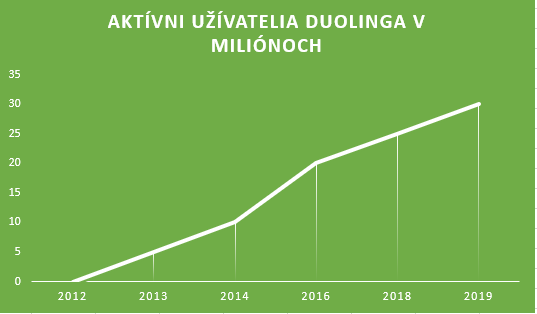
\includegraphics[width=\textwidth]{duolingo.png}
\caption{popis obrázka}
\label{duo-uzivatelia}
\end{figure}

Používanie aplikácie Duolingo je jednoduché a zameriava sa, na takmer všetky vekové kategórie\cite{duolingo}.
\subsection{Aplikácia Hellotalk} %3.2
HelloTalk je populárna aplikácia na trhu aplikácii na vzdelávanie jazyka. Hlavná myšlienka aplikácii je prepojiť užívateľa, ktorý sa chce naučiť daný jazyk s osobou, ktorej je daný jazyk rodný. HelloTalk má vela rôznych funkcií. Niektoré z nich sa odomknú až po zakúpení prémium verzii. Podľa webovej stránky HelloTalk aplikácia má sedem miliónov užívateľov.\cite{hellotalk}\\
Aplikáciou môžete zdielať: Hlasové správy, čety,  vzdielanie mobilnej kamery, vzdielanie čmáraníc, emotikony, zdielanie GPS lukácie a špecifické pomocné prvky na vzdelávanie jazyka (preklad, rozozanie hlasu, ...)\cite{hellotalk}.\\
\\
Výhody aplikácie HelloTalk:\cite{hellotalk}
\begin{itemize}
\item Možnosť bezpeňažného hovoru
\item Automatické prekladanie konverzácie (zabezpečuje plynulosť koverzácie)
\item Pomoc pri výslovnosti pri jazykoch, ktoré nepoužívaju latinskú abecedu
\end{itemize}
Nevýhody aplikácie HelloTalk:\cite{hellotalk}
\begin{itemize}
\item Nedostatočný systém na motivovanie užívateľa
\item Nie všetky funkcie su dostupné bez premium verzii
\item Žiadne spätná väzba pre užívatelov o ich postupe v učení 
\item Informovanie o čase v krajine osoby, ktorej píšem (odpoveď na otázku či je vhodné začať konverzáciu)
\end{itemize}

\subsection{Aplikácia Tandem}
Tandem je aplikácia založená na metóde výmeny jazykových znalostí, ktorá má korene v sedemdesiatych rokoch minulého storočia. Inak povedané, metológia vzdelávania aplikácia tandem je založená na koncepte rozhovoru medzi dvomi tandem partnermi (ideálne jeden z nich má daný jazyk ako rodný).
Zaujímavým prvkom tejto aplikácie je proces posúdenia nových uživateľov.\cite{tandem}

 Tandem je zameraný čisto len na jazykové účely a preto tento proces pomáha odstrániť nových užívateľov s inými záujmami. Proces posúdenia prebieha v podobe vyplnenia budúceho profilu užívateľa. Pri zadávaní profilovej fotografie vás aplikácia tandem automaticky upozorní, ak fotografia nespĺňa požadované kritériá \ref{tandem-obmedzenia}. Čas čakania na odsúhlasenie sa líši. Niektorí užívatelia boli odsúhlasený za pár dní ,iný týždne.\\

\begin{figure}[h] %obrázok
\centering

\includegraphics{tandem2.png}
\caption{Upozorenie po zadaní profilovej fotky, na ktorej nie je tvár}
\label{tandem-obmedzenia}
\end{figure}

Tandem je zložený z troch hlavných zložiek. Prvou je komunita, ktorá slúži na hľadanie vhodných tandem partnerov. Druhou sú platený učitelia. Kedže, tandem partneri sa nemôžu považovať za jazykových expertov, tak tandem umožňuje spojenie sa s učiteľmi jazyka. Poslednou sú čety, ktoré sú určené na prehľad a sumarizáciu konverzácii uživateľa.
\\

Výhody aplikácie Tandem: 
\begin{itemize}
\item Užívateľ si vie vybrať tandem partnera podľa spoločných záujmov uvedených v profile \cite{tandem}
\item Tandem partneri si vedia navzájom opraviť gramatiku prostredníctvom vstavanej funkcie
\item Tandem umožňuje videochaty \cite{tandem} a audio-správy
\item Užívatelia môžu filtrovať kto vidí ich profil a prerušiť kontakt s nežiadúcou osobou \cite{tandem}
\end{itemize}

Nevýhody aplikácie Tandem:
\begin{itemize}
\item Užívateľ musí mať aspoň základné porozumenie jazyka, ináč sa s tandem partnerom nedorozumie (avšak môže využiť služby učiteľov) \cite{tandem}
\item Veľa užívateľov využíva aplikáciu na zoznamovanie sa s novými ľuďmi, čo môže brániť vo vzdelávaní \cite{tandem}
\item Proces posudzovania profilu môže trvať dlho, veľa uživateľov sa na to sťažuje \cite{tandem}
\end{itemize}




\subsection{Jazykové blogy}
\cite{blog}
\cite{blog-mif}
\subsection{Online kurzy}

\section{Efektívnosť e-learningu}
\cite{duolingo}
\cite{efektivnost}
\section{Záver}

\bibliography{zdroje_literatura}
\bibliographystyle{plain}
\end{document}
